% !TEX root = ./report.tex

\clearpage
\section{Background}
\label{background}

\subsection{The Regionalized Value-State Dependence Graph}
\label{background:RVSDG}

The RVSDG is a Directed Acyclic Graph (DAG).

A RVSDG has different kinds of nodes, and two types of edges. Nodes can be
generalized into two categories, simple and complex nodes. Simple nodes are the
nodes representing the ``basic operations'' a program performs, such as the
addition and subtraction of integers. Complex nodes are nodes which contain an
RVSDG subgraph. The complex nodes presented below are the $\gamma$-, $\theta$-,
$\lambda$-, apply-, and $\phi$-nodes. The edges will be discussed first.

\subsubsection{Edges}

One type of edge used in an RVSDG is the data dependence edge. This edge
represents a data dependency one node has before it can be computed/executed.

The other type of edge is the state dependence edge. This edge is meant to keep
the ordering of the nodes consistent with the original flow of execution, when
there is no ordering by data dependencies between them. Stippled lines are
commonly used to denote state dependence edges.

\todo[inline]{Make tail-controlled $theta$-node example with some printfs for
showing state dependency edges?}

See Figure~\ref{missing_loop_figure_example?} for an example of why state
dependency edges are necessary for the RVSDG.

\subsubsection{Simple nodes}

Simple nodes are defined by their inability to contain an RVSDG subgraph.

Simple nodes are used in an RVSDG to represent simple operations, such as
addition, subtraction, and similarly simple operations often referred to as
\textit{primitive operations} in programming languages.

\subsubsection{Complex nodes}

\begin{itemize}

\item \textbf{N-way statements}

\textit{$\gamma$}-nodes represent conditional statements. Each $\gamma$-node has
two sets of inputs: the predicate, and all other edges its subgraph depend upon.

An if-statement is represented as a $\gamma$-node containing the subgraph
representing the body of the if-statement. If the predicate evaluates to true,
the subgraph will be executed.

If-else statements are also represented as $\gamma$-nodes, but they are
divided\footnote{Typically vertically.} into two subsections. One subsection of
the node contains the subgraph of what will happen if the predicate evaluates to
true, and the other will contain the subgraph representing the body of the else-
statement.

The equivalent of how an RVSDG representing nested if-statements looks like, is
shown with C/C++ in Listing~\ref{lst:nested_ifs}, and its representative RVSDG
example in Figure~\ref{fig:nested_ifs}.

\begin{center}
	\noindent\begin{minipage}{0.35\textwidth}
		\begin{lstlisting}[label={lst:nested_ifs}, style=customcpp,
caption={C/C++ code statements corresponding to Figure~\ref{fig:nested_ifs} to the
right.}]
if(smth){
	//do something 1
} else if(smth2){
	//do something 2
} else{
	//do something else
}
		\end{lstlisting}
	\end{minipage}
	\noindent\begin{minipage}{0.55\textwidth}
		\captionsetup{type=figure}
		\includegraphics[width=\textwidth]{figures/if_elseif_else_example}
		\captionof{figure}{Minimal example of two nested $\gamma$-nodes
representing the the same control flow as the code in
Listing~\ref{lst:nested_ifs} to the left.}
		\label{fig:nested_ifs}
	\end{minipage}
\end{center}

\item \textbf{Tail-controlled loops}

\textit{$\theta$}-nodes represent tail loops in the program. They are equivalent
to do-while loops containing the representation of the body of the loop. Like
with the $\gamma$-node, its inputs are all the dependencies needed by its
subgraph that represents the body of the loop.

Other loops, like for example for-loops, can be represented by putting a
$\theta$-node inside of the \textit{true} clause of a $\gamma$-node with an
empty subsection for the \textit{false} clause. If this textual example is to
represent a for-loop, both the $\theta$- and the $\gamma$-nodes need to each
have the same predicate.

\item \textbf{Functions}

\textit{$\lambda$}-nodes represent functions, and these are paired with
\textit{apply}-nodes. Their \textit{apply}-nodes represent the call sites of the
function in the graph (read: program). There should only exist one
$\lambda$-node per function in the program the RVSDG represents. As each
\textit{apply}-node represents a call site, all \textit{apply}-nodes have an
edge linking it to its corresponding $\lambda$-node.

See the $\lambda$- and its \textit{apply}-node inside of the $\phi$-node in
Fĩgure~\ref{fig:rec_fib_phi} for an example of a representation of a recursive
function in RVSDG.

\item \textbf{Mutually recursive functions}

\textit{$\phi$}-regions are nodes representing parts of the program's control
flow where functions behave recursively, either by calling themselves, or two or
more calling each other in turn (mutually recursive).

To uphold the DAG properties of an RVSDG, there is only one edge going from the
inner border of the $\phi$-node to the outer border of its contained
$\lambda$-node. Equivalently, an edge going out from the outer border of the
$\lambda$-node, to the inner edge of the $\phi$-node. This is to denote that
once the \textit{apply}-nodes have called the recursive function(s), the
function(s) will complete their execution inside of the $\phi$-node before
exiting the $\phi$-node. There is hence no cycle, and thus the DAG properties of
an RVSDG are upheld.

Figure~\ref{fig:rec_fib_phi} illustrates how a $\phi$-node containing the
representation of a recursive fibonacci function would look like in an RVSDG.

\end{itemize}

\begin{figure}[h]
	\centering
	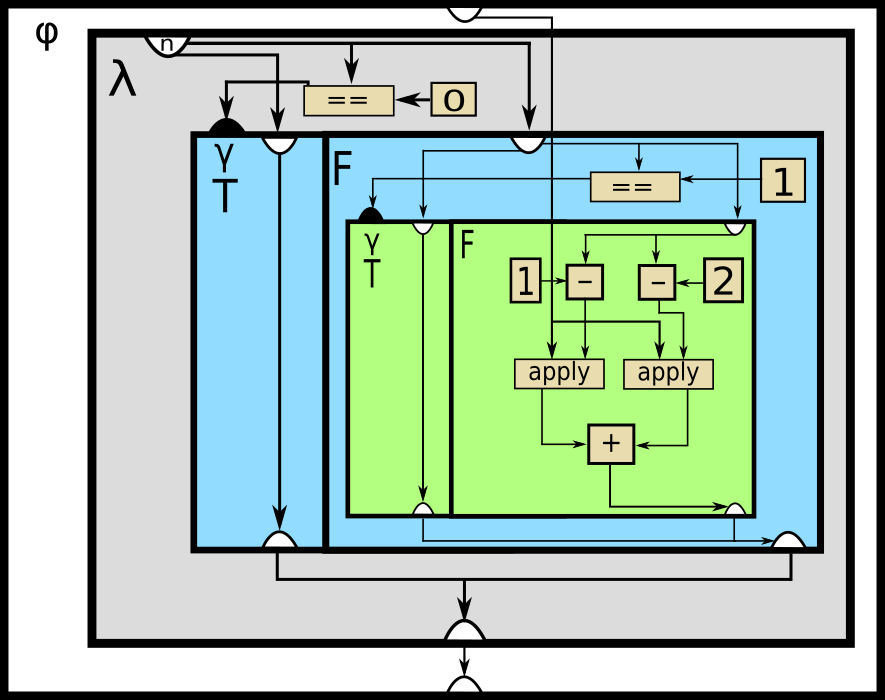
\includegraphics[width=0.75\textwidth]{figures/recursive_fibonacci}
	\caption{A $\phi$-node containing a $\lambda$-node representing a recursive
version of a function producing the $n$ first numbers in the Fibonacci series.}
	\label{fig:rec_fib_phi}
\end{figure}
